\chapter{CP}
A common scientific pattern, usually used to better understand a problem, is to decompose the case into
simpler and simpler parts that take in account just one or few aspects of the problem.
When we can control those aspect with a certain amount of reliability, we can mix different parts in order to
ensure that the superposition of those effects behaves as expected.
In this way we can build incremental models, that solve the problem by looking and optimizing a certain aspect
if the problem. 

\section{Base Model}
The \textbf{Base Model} is the most basic, where we defined our problem view, such as the parameters and the variables,
and we decided how to constraint it in order to get a satisfiable solution:

\begin{center}
    \begin{adjustwidth}{-1.5cm}{}
        \begin{tabular}{|c|c|c|}
            \hline
            \multicolumn{3}{|c|}{\textbf{Parameters}} \\
            \hline
            \textbf{Parameter} & \multicolumn{2}{|c|}{\textbf{Description}} \\
            \hline
            Width & \multicolumn{2}{|c|}{The Paper Sheet Width} \\
            \hline
            Height & \multicolumn{2}{|c|}{The Paper Sheet Height} \\
            \hline
            Presents & \multicolumn{2}{|c|}{The number of the Presents to place in the Paper Sheet} \\
            \hline
            Dimension X & \multicolumn{2}{|c|}{The array of the x dimensions of the Presents} \\
            \hline
            Dimension Y & \multicolumn{2}{|c|}{The array of the y dimensions of the Presents} \\
            \hline
            \multicolumn{3}{|c|}{\textbf{Extracted Parameters}} \\
            \hline
            \textbf{Parameter} & \textbf{Formula} & \textbf{Description} \\
            \hline
            Area & $Area = Width \cdot Height$ & Area of the Paper \\
            \hline
            Areas & $Areas[i] = Dimension_x[i] \cdot Dimension_y[i]$ & The array of the areas of the Presents \\
            \hline
            \multicolumn{3}{|c|}{\textbf{Variables}} \\
            \hline
            \textbf{Variable} & \multicolumn{2}{|c|}{\textbf{Description}} \\
            \hline
            Coord X &  \multicolumn{2}{|c|}{Array of the X positions of each Present} \\
            \hline
            Coord Y &  \multicolumn{2}{|c|}{Array of the Y positions of each Present} \\
            \hline
        \end{tabular}
    \end{adjustwidth}
\end{center}


\subsection{Main Problem Constraints}
Once the description of the problem is carried out, we defined some general constraints
in order to instruct the way to find a solution to the solver. The constraints are:

\begin{itemize}
    \item[] \textbf{Essential Constraints}
    \item \textbf{\textit{The presents must fit into the Paper Sheet:}}
        \begin{itemize}
            \item[] A present fits in the paper if its coordinates are strictly positive
                and its coorinates summed with its corresponding dimensions are lesser then
                the Paper Sheet dimensions.
            \item[] The resultant constraint is:
            \item[] $\forall i \in [1, Presents] \rightarrow\\(Coord_x[i] + Dimension_x[i] \leq Width + 1) \wedge \\ (Coord_y[i] + Dimension_y[i] \leq Height + 1)$  
            \item[] \textit{As we used indexes starting from 1, we must add 1 to the right side of both disequations} 
        \end{itemize}

    \item \textbf{\textit{Two different presents must not overlap:}}
        \begin{itemize}
            \item[] Given the two rectangles of two different presents, we can check if they have
                at least one part in common, just by checking their corners. So, we defined the
                \textit{overlaps} predicate:
            \item[] $overlaps(
                Left^1_x, Right^1_x, Left^1_y, Right^1_y,
                Left^2_x, Right^2_x, Left^2_y, Right^2_y
                ) \leftrightarrow
                \neg (Left^1_x \geq Right^2_x \vee Left^2_x \geq Right^1_x) \wedge\\
                \neg (Right^1_y \leq Left^2_y \vee Right^2_y \leq Left^1_y)$
            \item[] Each present is described as the rectangle:
            \item[] $Left^i_x, Left^i_y, Right^i_x, Right^i_y$
            \item[] So we can constraint each couple of presents to not overlaps one to each other:
            \item[] $
            \forall i, j \in [1, Presents], j > i \rightarrow\\
                \neg overlaps(\\
                    Coord_x[i], Coord_x[i] + Dimension_x[i], Coord_y[i], Coord_y[i] + Dimension_y[i],\\
                    Coord_x[j], Coord_x[j] + Dimension_x[j], Coord_y[j], Coord_y[j] + Dimension_y[j]\\
                )$ 
        \end{itemize}

        \begin{figure}
            \centering
            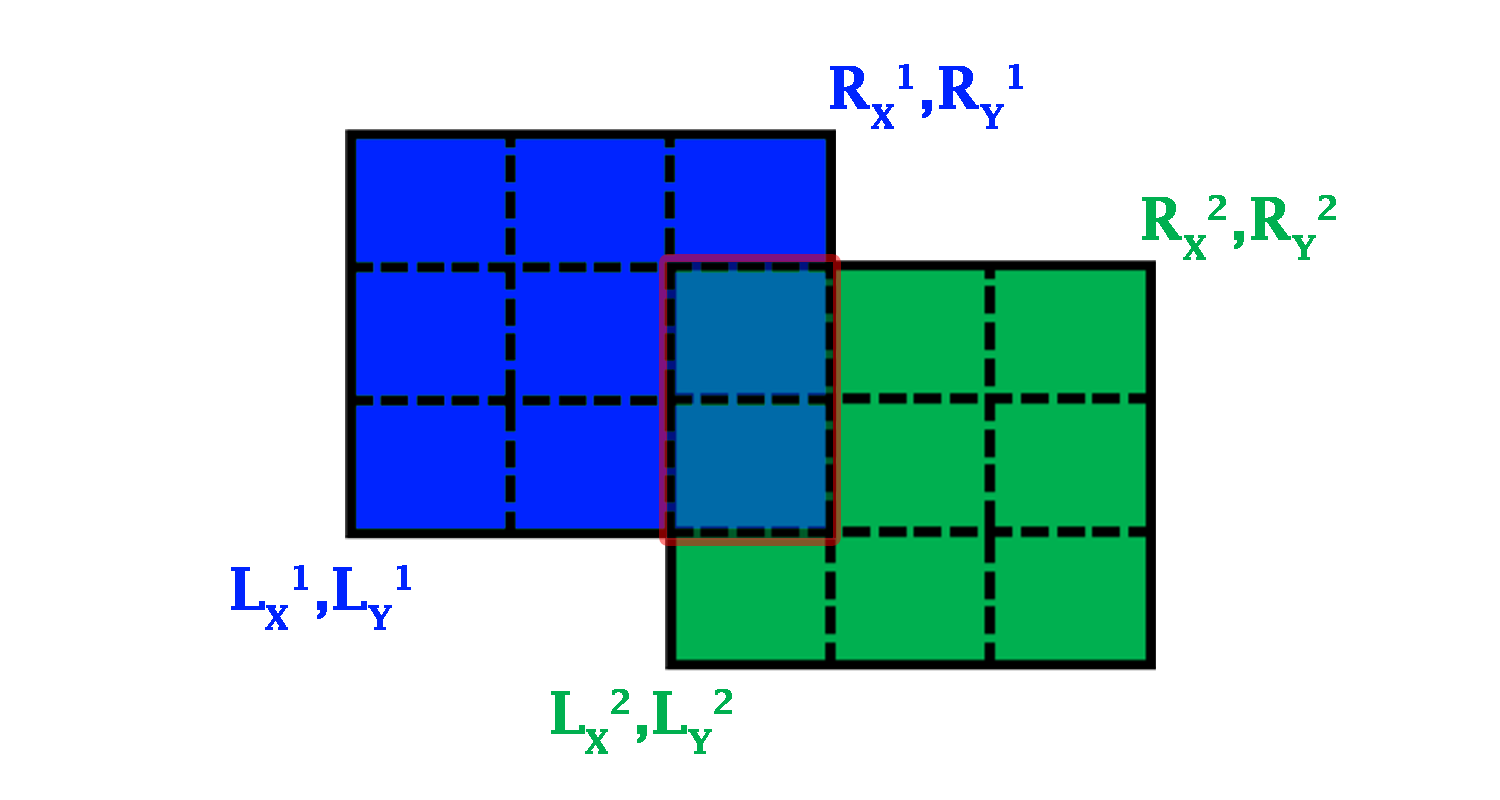
\includegraphics[width=\textwidth]{overlaps}
            \caption{Overlapping Model}
            \label{fig:overlaps}
        \end{figure}

    \item[] \textbf{Additional Constraints}
    \item[] These constraint are not essential to solve the general formulation of this problem,
        but they results helpful as they restrict the search space in the given instances.
        The underlying assumption is that the instance contains the right amount of presents such
        that the area of the Paper Sheet is completely used.
    \item \textbf{\textit{The total area of the presents must be the same of the Paper Sheet:}}
        \begin{itemize}
            \item[] $\sum_{i = 1}^{Presents}{Areas[i]} = Area$
            \item[] This constraint prevents the exploration of the search space
                at the very beginning. We indeed can instantly infer if the given instance is
                feasible: if the total areas does not match we can say the problem is unsatisfiable.
            \item[] A further relaxation of this constraint is to use $\leq$ instead of $=$ in order 
                to keep instances where we have presents that do not completely fill the Paper Sheet. 
                We kept the strict constraint for efficency reason, because the given instances all fall
                in this case.
        \end{itemize}
    \item \textbf{\textit{The presents must fill the row (column) dimension:}}
        \begin{itemize}
            \item[] As an extension of the previous constraint, we want to use each row \textit{(or column)}
                such that we use all of the available area of the paper.
            \item[] Drawing a vertical \textit{(horizontal)} line and summing up the encountered
                presents dimensions we must end up with the same dimension of the Paper Sheet:
            \item[] Rows: $
                \forall y \in [1, Height] \rightarrow\\ \sum_{i = 1}^{Presents}{
                    \begin{cases}
                    Dimension_x[i] & \text{if } y \geq Coord_y[i] \wedge y < Coord_y[i] + Dimension_y[i] \\
                    0 & \text{otherwise}
                    \end{cases}
                    }\\= Width$
            \item[] Columns: $
                \forall x \in [1, Width] \rightarrow\\ \sum_{i = 1}^{Presents}{
                    \begin{cases}
                    Dimension_y[i] & \text{if } x \geq Coord_x[i] \wedge x < Coord_x[i] + Dimension_x[i] \\
                    0 & \text{otherwise}
                    \end{cases}
                    }\\= Height$
        \end{itemize}
\end{itemize}

\subsection{Search Methods}
All of the constraints we described so far could solve the given instances with the \textit{Geocode} solver,
but the main difficulty is the time spent in the resolution. Some instances can take more then 10 minutes.
To lower the elasped time, we can tell to the solver how to optimize the search on the variables:
\begin{itemize}
    \item We decided to choose a preferential axes for the search. The X axis was choosen.
    \item Each axis then can be explored in different ways. We want to explore it with the most difficult case
        as we already know that some presents configurations can exclude a priori the placement of other presents.
        In this way we selected the \textit{\textbf{first\_fail}} search parameter, that chooses the variable with
        the smallest domain and try to find out if can have a value in the current solution state.
        If there are no possible values, we prevented the solver to search useless branch of the search tree.
        As we place presents into the sheet, each variable will lose a part of its domain, so we will choose that
        one that is most likely to fail.
    \item Now we must select an heuristic that chooses intelligently a value for the given variable. Our problem
        description has coordinates of each presents in their lower left corner, so we try to assign first the lesser
        available coordinates, then the bigger one. The \textit{\textbf{indomain\_min}} search parameter try to assign
        to each variable the minimum value available in the current domain.
    \item The final search annotiation is:
    \item[] $seq\_search([\\
            \text{\ \ \ \ }int\_search(Coord\_X, first\_fail, indomain\_min),\\
            \text{\ \ \ \ }int\_search(Coord\_Y, first\_fail, indomain\_min)\\
        ])$
\end{itemize} 

We also tried any combination of all the possible parameters in order to confirm our reasoning, so we end up by choosing
this setup because it resulted the most performant.

\section{Symmmetry Model}
We had further analysed the problem in order to understand if, from an erroneous solution,
there are similar solutions that we can deduce as unsatisfiable as they are permutation or simmetrical of the
erroneous one. This technique is called \textbf{Symmetry Breaking}.\\
The \textbf{Present Wrapping Problem} \cite{project} is an extension of the \textbf{2D Bin Packing Problem},
and one of the most effective heuristic to place presents is to choose those that are more restricting for the others,
in other words, the bigger the present is, the most difficult is to place, the more it will restrict the other presents
domains and the more effective will be its placement in the first stages. So the best analytical and empirical heuristic
found so far for this kind of problem is to sort the presents in size order, placing the bigger first and the
smaller last \cite{binpack, algdesign}.\\
Doing this requires a new extracted parameter:

\begin{center}
    \begin{adjustwidth}{-1.5cm}{}
        \begin{tabular}{|c|c|c|}
            \hline
            \multicolumn{3}{|c|}{\textbf{Extracted Parameters}} \\
            \hline
            \textbf{Parameter} & \textbf{Formula} & \textbf{Description} \\
            \hline
            Sorted Areas Indexes & \makecell{$Sorted\_Areas\_Indexes =$ \\ $reverse(arg\_sort(Areas))$} & Indexes of the Areas sorted by Present Area \\
            \hline
        \end{tabular}
    \end{adjustwidth}
\end{center}

This new parameter stores the indexes of the sorted areas, so the $Sorted\_Areas\_Indexes[1]$ will store the indexes of the present with
the maximum area, $Sorted\_Areas\_Indexes[2]$ the index of the second present with maximum area and so on.\\
Now the most basic constraint we can add is that the biggest present will always stay on the minimal coordinates:\\
$
Coord\_X[Sorted\_Areas\_Indexes[1]] = 1\\
Coord\_Y[Sorted\_Areas\_Indexes[1]] = 1
$
\\

Then we want to place the bigger presents in the left-bottom most part of the paper, simulating the fact that we are placing them before
the others:\\
$
\forall i, j \in [1, Presents], j > i \rightarrow \\
    Coord_y[Sorted\_Areas_Indexes[i]] = Coord_y[Sorted\_Areas\_Indexes[j]] \rightarrow \\
    Coord_x[Sorted\_Areas_Indexes[i]] < Coord_x[Sorted\_Areas\_Indexes[j]]
$
\\
This, in combination with the search method, provides that the bigger present will be then the lesser will be its coordinate x,
and since the bigger the present, the smaller is its domain, it will be also placed first, that means in the lower y possible.
By doing this we can exclude all the possible symmetries due to the swap of different area presents.\\
Excluding the symmetrical solutions allow us to exclude also the symmetrical part of the search tree that are unsatisfiable, just
by finding an unsatisfiable combination out of the all simmetricals.

% TODO: Example Image

\section{Rotation Model}
% TODO

\section{Symmetry Rotation Model}
As we growth the model in modules, we can just combine the \textbf{Symmetry Model} with the \textbf{Rotation Model} and we end up
with a \textbf{Symmetry Rotation Model} that takes in account the possibility of the presents rotation and also excludes the symmetrical
solutions.

\section{Duplicated Symmetry Model}
Another point to take in account, is the possibility of the presence of presents that have the same size. As we modelled the problem,
the \textbf{Base Model} can already solve this kind of instances, but we can add some constraints in order to exploit the Symmetry Breaking
even in these cases.

% TODO

\section{Duplicated Symmetry Rotation Model}
The modularity of our model eassily achieves a new model that takes in account all the discussed properties of the problem
\textit{(Symmetry, Rotation, Duplicated Presents)} at once, just by combining the constraints of all the precedent models.
The results show that this model achieve the best performance, as the number of errors and the quantity of the explorated nodes in the
search tree drastically decrease.  

\section{Remarks}
% TODO
% TODO: Geocode and Chuffed diffrences